\chapter{Implementácia}

V tejto kapitole si popíšeme dôvody pre výber jazyka a knižníc a niektoré časti nášho zarovnávača.

\section{Výber jazyka a použité knižnice}
%daky pokec o~tom ze som to pisal v~pythone a preco je python super
Ako jazyk pre písanie nášho zarovnávača sme si vybrali Python (vo verzii 2.7). Dôvodov sme mali niekoľko: V prvom rade zarovnávač sme nepísali od začiatku, ale ako základ sme zobrali zarovnávač od Michala Nánásiho (viď sekcia \ref{subsec:realigner}), ktorý už bol napísaný v jazyku Python 2.7. Ďalšími dôvodmi sú pohodlnosť písania v jazyku Python a dostupnosť veľkého množstva užitočných knižníc. Knižnice pre Python sa dajú písať aj v jazyku C alebo C++, čo umožňuje skĺbiť rýchlosť C a jednoduchosť jazyka Python.

\subsection{Realigner}
\label{subsec:realigner}

\textit{Realigner} je zarovnávač, ktorý napísal Michal Nánási pre potreby \cite{nanasi2013probabilistic}. Umožňuje prezarovnanie\footnote{modifikáciu existujúceho zarovnania} sekvencií pomocou párových HMM a Viterbiho algoritmu. Prezarovnanie dokáže robiť aj vrámci lokálneho okolia okolo pôvodného zarovnania. Program je rozšíriteľný o nové modely, čo sme využili pre naše potreby.

\subsection{Pythonové knižnice}
%  python kniznice - najma scikit-learn, numpy, track
V našom programe sme sa rozhodli využiť niekoľko knižníc. Najdôležitejšími boli knižnice \textit{numpy}, \textit{scipy}, \textit{scikit-learn}, \textit{pyplot}, \textit{track} a \textit{pandas}.

Numpy je matematická knižnica, ktorá obsahuje množstvo užitočných matematických funkcií. Pre nás z nej boli dôležité hlavne štatistické funkcie, napr. generovanie náhodných čísel z rôznych rozdelení a počítanie štandardnej odchýlky. Okrem toho je táto knižnica základom aj pre väčšinu ostatných knižníc.

Scipy obsahuje funkcie pre pokročilejšie vedecké výpočty. My sme z nej využili hlavne funkciu na odhad rozdelenia pomocou gausiánov.

Scikit-learn je knižnica zaoberajúca sa hlavne strojovým učením. Odtiaľ sme využili náhodné lesy.

Pyplot je knižnica na kreslenie grafov a využili sme ju na vygenerovanie všetkých našich vizualizácií.

Track je knižnica na prácu s {\tt '.bed'} súbormi, v ktorých sme mali uložené naše anotácie.

Pandas je knižnica na analýzu a úpravu veľkých dát. Poslúžila nám najmä pri príprave anotácií pre biologické zarovnania.

\section[Triedy na zarovnávanie s klas.]{Triedy na zarovnávanie s~klasifikátorom}

V tejto sekcii si popíšeme najdôležitejšie triedy, ktoré sme doplnili do programu Realigner. Ide o triedy na presdpracovanie dát, klasifikáciu a triedy pre stavy pHMM.

\subsection{Predspracovanie dát}

\todo obrazok classdiagramu

Na predspracovanie dát nám slúžili triedy \textit{DataPreparer}, \textit{ComparingDataPreparer}, \textit{FullComparingDataPreparer}, \textit{CombinedDataPreparer},
\textit{IndelDataPreparer}, \textit{ComparingIndelDataPreparer}, \textit{FullComparingIndelDataPreparer} a \textit{CombinedIndelDataPreparer} (obr \ref{fig:classdiagram-preparers}).

Trieda DataPreparer je rodičovskou triedou pre ostatné triedy, takže si popíšeme najmä ju. Trieda IndelDataPreparer je rodičom Indel verzií tried. Triedy majú dve hlavné úlohy: Prvá je predpríprava dát na klasifikáciu a druhá je predspracovanie trénovacej množiny.

Pri predpríprave dát je úlohou dať dáta do formy vhodnej pre klasifikátor. To znamená získať okno a anotácie a ďalšie atribúty tak ako sme ich popísali v kapitole \ref{subsec:attribute-selection}. Naše štyri typy tried sa líšia iba v tejto úlohe a zodpovedajú štyrom typom dát. Najdôležitejšia práca sa vykoná v metóde \method{\_prepare\_sequence}, ktorá pripraví dáta pre jednu sekvenciu, a potom zlepia dáta z volania tejto funkcie pre obe sekvencie. Indel verzie tried obsahujú príslušné úpravy aby v sekvencii s medzerou použili kratšie okno.

Pri predspracovaní trénovacej množiny treba zo zarovnaní vytvoriť pozitívne a negatívne príklady. Táto metóda je implementovaná len v DataPreparer a IndelDataPreparer triede, ostatné ju zdedia. Pri výbere pozitívnych príkladov v triede DataPreparer označujeme pozície v sekvencii, ktoré sú zarovnané. To má na starosti metóda \method{prepare\_positive\_data}. Metóda \method{prepare\_negative\_data} vyberá negatívne príklady použitím zarovnaných pozícií z pozitívnych príkladov a náhodne ich poposúva podľa vzorca spomenutého v sekcii \ref{subsec:clf-training}. Okrem toho sme implementovali aj alternatívny výber negatívnych dát v metóde \method{prepare\_negative\_data\_random}, kde negatívne príklady vyberáme náhodne z nezarovnaných pozícií s tým, že vyberieme rovnako veľa negatívnych ako pozitívnych príkladov. V Indel klasifikátore sa oba typy príkladov vyberajú v metóde \method{prepare\_training\_data}, pričom jedna sekvencia sa zvolí za medzerovú a za pozitívne príklady sa vezme všetko čo je zarovnané k medzere v medzerovej sekvencii. Za negatívne sa vezme rovnako veľa náhodných zarovnaných pozícií.

\subsection{Abstrakcia klasifikátora}
\label{subsec:pairclassifier}
V pre väčšiu modularitu sme sa rozhodli naprogamovať vrstvu medzi klasifikátorom a zvyškom programu. Trieda sprostredkúvajúca túto vrstvu sa volá \textit{PairClassifier}. Poskytuje metódy také ako klasifikátor a niekoľko navyše.

Jej hlavnými výhodami sú:

\begin{itemize}
    \item možnosť rýchlej výmeny klasifikátora bez úpravy zvyšku programu
    \item automatické predspracovanie pri klasifikácii a trénovanií pomocou príslušnej triedy DataPreparer
    \item automatické trénovanie -- ak klasifikátor nie je natrénovaný, tak sa automaticky natrénuje z prednastavenej trénovacej množiny
    \item hromadná klasifikácia s predspracovaním
    \item otočenie výstupu klasifikátora
\end{itemize}

\subsection{HMM stavy s~klasifikátorom}
\label{subsec:hmm-states}

V zarovnávači bol implementovaný Viterbiho algoritmus, ktorý pracoval s párovými HMM. Tento algoritmus pracoval s triedou \textit{GeneralizedPairState}, ktorá poskytovala metódu \method{emission} vracajúcu emisiu báz na daných pozíciách. Od tejto triedy dedia naše triedy \textit{ClassifierState}, \textit{ClassifierIndelState} a preťažili sme metódu \method{emission} tak, aby vracala hodnoty z klasifikátora. Museli sme však urobiť niekoľko zmien. Viterbiho algoritmus si pýta emisie po jednej. Avšak volanie C-čkovej funkcie z knižnice scikit-learn z Pythonu je pomalé, takže pre dlhé sekvencie by zarovnanie trvalo veľmi dlho. Preto sme si najskôr naraz počas jedného volania funkcie predpočítali emisie pre všetky pozície a tie sme potom vracali v momente, keď si ich Viterbiho algoritmus vypýtal. Na to sme využili možnosť hromadnej klasifikácie v našej triede PairClassifier (sekcie \ref{subsec:pairclassifier}). Tieto dve triedy sa líšia iba v použitej triede na predspracovanie dát.

Od tried ClassifierState a ClassiFierIndelState potom dedia triedy \textit{ClassifierAnnotationState} a \textit{ClassifierAnnotationIndelState}, ktoré tvoria diskrétnu verziu nášho modelu B. Triedy mali v súbore uložené tabuľky emisií a podľa aktuálnych pozícií si zistili bázy a aktuálny výstup klasifikátora, ktoré slúžili ako indexy do tabuľky. Tieto triedy navyše obsahujú metódy trénovanie emisií.

Od tried ClassifierAnnotationState a ClassifierAnnotationIndelState dedia triedy \textit{ContignuousClassifierAnnotationState} a \textit{ContignuousClassifierAnnotationIndelState}, ktoré stvárňujú spojitú verziu modelu B. Tieto triedy majú v tabuľke emisií pre každú dvojicu báz uloženú serializovanú verziu objektu \textit{gaussian\_kde}, ktorý tvorí distribúciu výstupu klasifikátora. Konkrétnu hodnotu potom získa volaním príslušného objektu k danej dvojici báz (resp. báze pri IndelState) s hodnotou klasifikátora. Tieto triedy takisto obsahujú aj metôdy na trénovanie emisií.

Od triedy \textit{GeneralizedPairState} navyše dedia aj naše triedy pre referenčný model -- \textit{SimpleMatchState} a \textit{SimpleIndelState}, triedu GeneralizedPairState rozširujú o metódy na trénovanie emisných pravdepodobností.

\todo obrazok classdiagramu

\section{Pomocné programy}
\subsection{Simulátor}

Simulátor slúži na overenie funkčnosti zarovnávača. Náhodne vygeneruje 2 sekvencie, ktoré vznikli zo spoločného predka a vyrobí korektné zarovnanie. Okrem toho vyrobí aj nejaké dodatočné informácie ktoré majú pomôcť pri zarovnávaní.

\subsubsection{Algoritmus}
Simulátor vygeneruje informáciu o~tom, ktoré časti sekvencie prislúchajú génom a ktoré nie. Informácia má podobu boolovského vektora.
Simulátor najskôr vygeneruje \textit{základnú (master) postupnosť} a z~nej odvodí dve ďalšie postupnosti, ktoré zodpovedajú sekvenciám.

Okrem toho simulátor vygeneruje dve sekvencie, pričom prvú vyrobí náhodne a druhú odvodí z~nej pomocou mutácie a inzercie/delécie.
V~našom prípade sme inzerciu vynechali a simulujeme ju ako deléciu v~druhej sekvencii.
Pri odvodzovaní bude používať aj informáciu o~tom, ktorá časť je gén a ktorá nie.

Keďže simulátor vie spôsob akým generoval druhú sekvenciu z~prvej, vie aj korektné zarovnanie.

Simulátor má vopred daných niekoľko konštánt -- pravdepodobnosti udalostí, ktoré môžu nastať.

\subsubsection{Generovanie informácie o~génoch}
Ak sa na danom mieste nachádza gén, označíme to $1$ inak $0$.
Gény bývajú súvislé úseky, takže ich treba generovať tak, že niekedy začneme gén, potom generujeme 1, potom skončíme gén a generujeme 0. Potom môžme opäť začať gén atď.

\begin{figure}[htp]
    \centering
    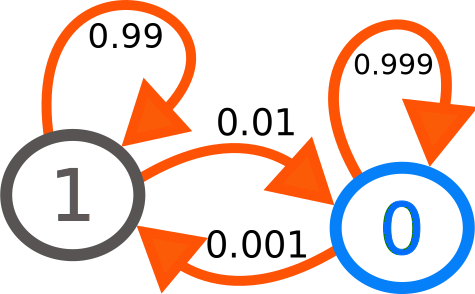
\includegraphics[width=.3\textwidth]{images/markov_chain}
    \caption{Markovova reťaz použitá na generovanie informácie o~génoch}
    \label{fig:markov-chain}
\end{figure}

Generovanie robíme pomocou \textit{Markovovskej reťaze (Markov Chain)} obr. \ref{fig:markov-chain}. Generujeme podľa aktuálneho stavu a v~každom kroku sa podľa pravdepodobnosti rozhodneme či sa prepneme do iného stavu alebo ostaneme v~tom istom. Rozhodnutie robíme pomocou \textit{falošnej mince (biased coin)}, kde hlava padne s~určitou pravdepodobnosťou, ktorú vopred nastavíme.

%TODO ak bude treba zabrat miesto, tak sem drbnut nejake zdrojaky

Máme vygenerovanú master postupnosť a z~nej teraz vyrobíme dve postupnosti pre sekvencie tak, že skopírujeme master sekvenciu, pričom každú 1 s~určitou pravdepodobnosťou (v~našom prípade $0,1$) zmeníme na 0.

\subsubsection{Simulácia mutácie}

Máme vygenerovanú sekvenciu a ideme vyrobiť zmutovanú sekvenciu. Spravíme to tak, že s~určitou pravdepodobnosťou sa nahradí báza z~pôvodnej sekvencie inou bázou. Pravdepodobnosť závisí aj od toho, či je na danej pozícii gén v~oboch sekvenciách, v~jednej, alebo v~žiadnej. Na rozhodnutie používame jednu z~troch falošných mincí podľa toho, ktorá z~možností nastala (gén v~oboch sekvenciách, v~jednej, alebo žiadnej).

\subsubsection{Simulácia delécie}
Deléciu simulujeme opäť pomocou Markovovskej reťaze, pretože pri evolúcii majú tendenciu vypadávať súvislé úseky. Pravdepodobnosť, že začneme mazať je $0,01$ a že prestaneme $0,1$.
Ak mažeme, nahradzujeme danú bázu znakom {\verb+'-'+}.

\subsubsection{Využitie}

Simulátor je prvá vec, ktorú sme implementovali a slúžil na väčšinu našich experimentov. Simulované dáta majú totiž oproti biologickým niekoľko výhod. Prvou je, že poznáme správnu odpoveď a teda môžme objektívne zhodnotiť úspešnosť našich modelov. Druhou je možnosť zvoliť si parametre, ktoré menia závislosť mutácií na anotácii a testovať, správanie modelov ak zvýšime túto závislosť. Ďalšou výhodou je, že si môžme vygenerovať ľubovoľne veľa ľubovoľne dlhých sekvencií.

\subsection{Trénovanie modelov}

Trénovanie modelov má na starosti trieda \textit{ModelTraining} a je urobené pomocou metódy maximálnej vierohodnosti (kapitola \ref{subsec:hmmtraining}).
Trénovanie prechodových pravdepodobností je pre všetky modely spoločné. Trénovanie emisných pravdepodobností má každý stav spravené zvlášť, pretože stavy emitujú rôzne symboly.
Trieda ModelTraining najskôr načíta model z ktorého zistí stavy.
Potom načíta trénovacie sekvencie a oanotuje ich stavmi. Následne vypočíta prechodové pravdepodobnosti. Spočíta všetky výskyty nasledujúcich stavov vo všetkých sekvenciách pre každý stav zvlášť. To vydelí celkovým počtom výskytov daného stavu. Potom oanotované sekvencie predloží jednotlivým stavom, aby vypočítali emisné pravdepodobnosti.

Máme štyri základné typy stavov, ktoré sme si popísali v časti \ref{subsec:hmm-states}:
\begin{itemize}
    \item SimpleMatchState, SimpleIndelState
    \item ClassifierState, ClassifierIndelState
    \item ClassifierAnnotationState, ClassifierAnnotationIndelState
    \item ContignuousClassifierAnnotationState, ContignuousClassifierAnnotationIndelState
\end{itemize}

V SimpleMatchState, SimpleIndelState je algoritmus priamočiary spočíta výskyty príslušných dvojíc báz (resp. báz) a vydelí celkovým počtom výskytu stavu.
V ClassifierState, ClassifierIndelState sa emisie netrénujú, takže tabuľka bude prázdna.
V ClassifierAnnotationState, ClassifierAnnotationIndelState sa pre každý stav a pre každú dvojicu báz (resp. bázu) spočítajú hodnoty z klasifikátora a tie sa následne aproximujú pomocou gausiánov. Na toto využijeme funkciu \method{gaussian\_kde} z modulu \method{scipy.stats}. Táto metóda robí odhad distribučnej funkcie a má parameter -- šírku pásma. Šírku pásma sme nechali na predvolenej hodnote -- "scott". Tá nastavuje šírku pásma podľa vzorca:
$$n^{-1/(d+4)},$$
kde $n$ je počet vstupov a $d$ je počet dimenzií (v našom prípade $d = 1$). Viac detailov je v \cite{scipydoc} alebo \cite{wiki:kde}. Následne túto funkciu diskretizujeme na $k$ hodnôt. To spravíme pomocou určitého integrálu, na čo nám slúži metóda \method{integrate\_box(a, b)}, ktorá spočíta určitý integrál od $a$ po $b$.
Keďže gaussian\_kde je definovaný na intervale $\left<-\infty, \infty \right>$ a $$\int_{-\infty}^\infty \! gaussian\_kde(x) \mathrm{d}x = 1,$$ orezaním definičného oboru na $\left<0,1\right>$ sa môže stať, že $$\int_0^1 \! gaussian\_kde(x) \mathrm{d}x < 1.$$ V tom prípade výslednú hodnotu ešte musíme normalizovať vydelením hodnotou $$norm = \int_0^1 \! gaussian\_kde(x) \mathrm{d}x.$$ Ako sme si ukázali v \ref{sec:model-training} výslednú pravdepodobnosť dopočítame vynásobením diskretizovanej pravdepodobnosti daného výstupu klasifikátora v prípade daných báz a pravdepodobnosti daných báz.
V ContignuousClassifierAnnotationState, ContignuousClassifierAnnotationIndelState postupujeme rovnako ako v predchádzajúcom prípade, ale distribúciu už nediskretizujeme. Namiesto toho si ju uložíme do súboru ako $g$ spolu s číslom $p/norm$, kde $p$ je pravdepodobnosť daných báz a $norm$ je normalizačná konštanta -- tá istá ako v predchádzajúcom prípade. Hustotu emisie potom v stave vypočítame tak, že zoberieme parametre pre danú dvojicu báz (resp. bázu) -- $g$ a $p/norm$ -- a pre výstup klasifikátora $c$ bude hustota $g(c)*p/norm.$
% \subsection{Testovanie klasifikátora}
% \todo random\_forest\_evaluation.py

\section{Použitie}
\todo v~kratkosti o~tom ako to vobec spustit so svojimi sekvenciami a modelmi...

\todo mozno sem dat aj moznosti rozsirenia

\todo konfiguracia - constants.py a config.py
